\section{What the Rolling Persistence State Measures}\label{sec:window}

\subsection{The state}

For each stock and weekly origin, $\hat d_{i,t}(W)$ denotes the GPH estimate
computed from the $W$ log-variance observations ending on day $t$, with
$W=750$ in the baseline. The persistence state is the cross-sectional mean
$\bar d_t(W) = N^{-1}\sum_i \hat d_{i,t}(W)$, together with its
cross-sectional standard deviation. The state rises sharply in crises: it
averages about 0.38 in calm years and 0.57 while the 2020 episode is inside
the window. Read as a property of the market, this would mean that shocks to
volatility became markedly more persistent after March 2020 and remained so
for three years.

\subsection{A mechanical account}

A simpler account predicts the same rise and makes three further predictions
that the persistence interpretation does not. Suppose that log variance is a
short-memory process plus a temporary episode, a block of elevated values of
height $b$ and length $L$. Within a window of length $W$, the episode adds a
component to the discrete Fourier transform whose modulus at the Fourier
frequency $\lambda_j = 2\pi j/W$ is
$b\,\lvert\sin(L\lambda_j/2)/\sin(\lambda_j/2)\rvert$. This modulus is large
at frequencies below about $2\pi/L$ and does not depend on the position of
the episode within the window, because shifting the episode changes only the
phase. The log-periodogram estimator regresses the log periodogram on log
frequency over the lowest $m$ frequencies, so the additional low-frequency
power raises $\hat d$. Three predictions follow. First, the estimate jumps
when the episode enters the window, stays roughly constant while the episode
is inside, and falls when it leaves; the fall therefore occurs $W$ days after
the episode and moves one-for-one with the window length. Second, the size
of the effect increases with the duration of the episode, not only with its
peak, so a one-day crash should have little effect. Third, the state should
track the largest recent episode more closely than the current level of
volatility. None of these predictions requires the persistence of shocks to
change.

\subsection{Evidence}

The events are fixed in advance as the three largest days of cross-sectional
mean log variance that lie at least 250 trading days apart: 10 October 2008,
6 May 2010 (the Flash Crash) and 18 March 2020. For each event and window
length $W\in\{500, 750, 1000\}$, Panel A of Table~\ref{tab:window} compares
the mean state over the four weeks after the event day enters the window
with the mean over the four weeks before, and does the same when the day
leaves the window $W$ trading days later. Each change is ranked among all
four-week changes in the series.

\begin{table}[H]
\caption{What the rolling persistence state tracks.}
\label{tab:window}
\footnotesize
\begin{tabularx}{\textwidth}{lXXXXXX}
\toprule
\multicolumn{7}{l}{\textit{Panel A. Change in $\bar d_t(W)$ when the event day enters and leaves the window (percentile among all changes)}} \\
\midrule
Event & $W$ & Entry & Pct & Exit date & Exit & Pct \\
\midrule
2008-10-10 & 500 & +0.159 & 99.8 & 2010-10-06 & +0.009 & 80.8 \\
 & 750 & +0.093 & 99.6 & 2011-10-03 & -0.065 & 0.8 \\
 & 1000 & +0.104 & 99.5 & 2012-09-28 & -0.036 & 1.7 \\
2010-05-06 & 500 & -0.008 & 22.7 & 2012-04-30 & -0.000 & 51.6 \\
 & 750 & +0.012 & 90.4 & 2013-04-30 & -0.017 & 9.6 \\
 & 1000 & +0.002 & 65.9 & 2014-04-28 & -0.022 & 5.4 \\
2020-03-18 & 500 & +0.181 & 99.9 & 2022-03-11 & -0.164 & 0.2 \\
 & 750 & +0.125 & 99.9 & 2023-03-10 & -0.108 & 0.1 \\
 & 1000 & +0.108 & 99.7 & 2024-03-08 & -0.090 & 0.1 \\
\midrule
\multicolumn{7}{l}{\textit{Panel B. $R^2$ of $\bar d_t(W)$ on the VIX}} \\
\midrule
& $W$ & \multicolumn{2}{c}{Max VIX in window} & & \multicolumn{2}{c}{Current VIX} \\
\midrule
& 500 & \multicolumn{2}{c}{0.81} & & \multicolumn{2}{c}{0.28} \\
& 750 & \multicolumn{2}{c}{0.83} & & \multicolumn{2}{c}{0.27} \\
& 1000 & \multicolumn{2}{c}{0.82} & & \multicolumn{2}{c}{0.18} \\
\midrule
\multicolumn{7}{l}{\textit{Panel C. The 2020 episode: data versus a short-memory null}} \\
\midrule
& $W$ & Before & Inside & After exit & Rise & Largest drop \\
\midrule
Data & 500 & 0.35 & 0.60 & 0.33 & +0.25 & \\
Null & 500 & 0.41 & 0.54 & 0.47 & +0.13 & day 509 \\
Data & 750 & 0.38 & 0.57 & 0.33 & +0.19 & \\
Null & 750 & 0.40 & 0.53 & 0.46 & +0.13 & day 759 \\
Data & 1000 & 0.37 & 0.53 & 0.34 & +0.16 & \\
Null & 1000 & 0.39 & 0.50 & 0.44 & +0.11 & day 1009 \\
\bottomrule
\end{tabularx}
\noindent{\footnotesize{\textit{Notes:} $\bar d_t(W)$ is the cross-sectional mean of the GPH estimate on log Parkinson variance over the $W$ trading days ending on day $t$, on the weekly grid. Events are the three largest days of cross-sectional mean log variance at least 250 days apart (rule fixed in advance). Entry and exit changes compare the four weekly estimates after the date with the four before; Pct is the percentile of that change among all such changes. Panel C: mean $\bar d_t$ in the 120 days before the event, from day 60 to day $W-60$, and from day $W+20$ to $W+120$. The null is an ARMA(1,1) with the median parameters of per-stock fits to 2012--2019 log variance plus the observed one-year 2020 excess log variance, 200 replications; Largest drop is the day (relative to the event) of its largest four-week fall.}}
\end{table}


The 2020 event produces the predicted pattern at every window length. The
state rises by 0.11 to 0.18 on entry, among the largest 0.3\% of changes, and
falls by 0.09 to 0.16 on exit, among the smallest 0.2\%. The exit dates are
11 March 2022, 10 March 2023 and 8 March 2024. Figure~\ref{fig:window} shows
the three series: each holds a plateau and drops on its own exit date. The
October 2008 event shows the same pattern at 750 and 1000 days. At 500 days
its exit is masked because the remainder of the 2008--2009 episode and the
May 2010 turmoil are still inside the window. The Flash Crash, a single
extreme day, barely moves the state on entry or exit, as the second
prediction requires.

Panel B tests the third prediction. The largest VIX close inside the same
window explains 81--83\% of the variation in the state at every window
length, whereas the current VIX explains 18--28\%. Most of the variation in
the state is therefore accounted for by a single observable, the highest VIX
close in the estimation window.

\begin{figure}[H]
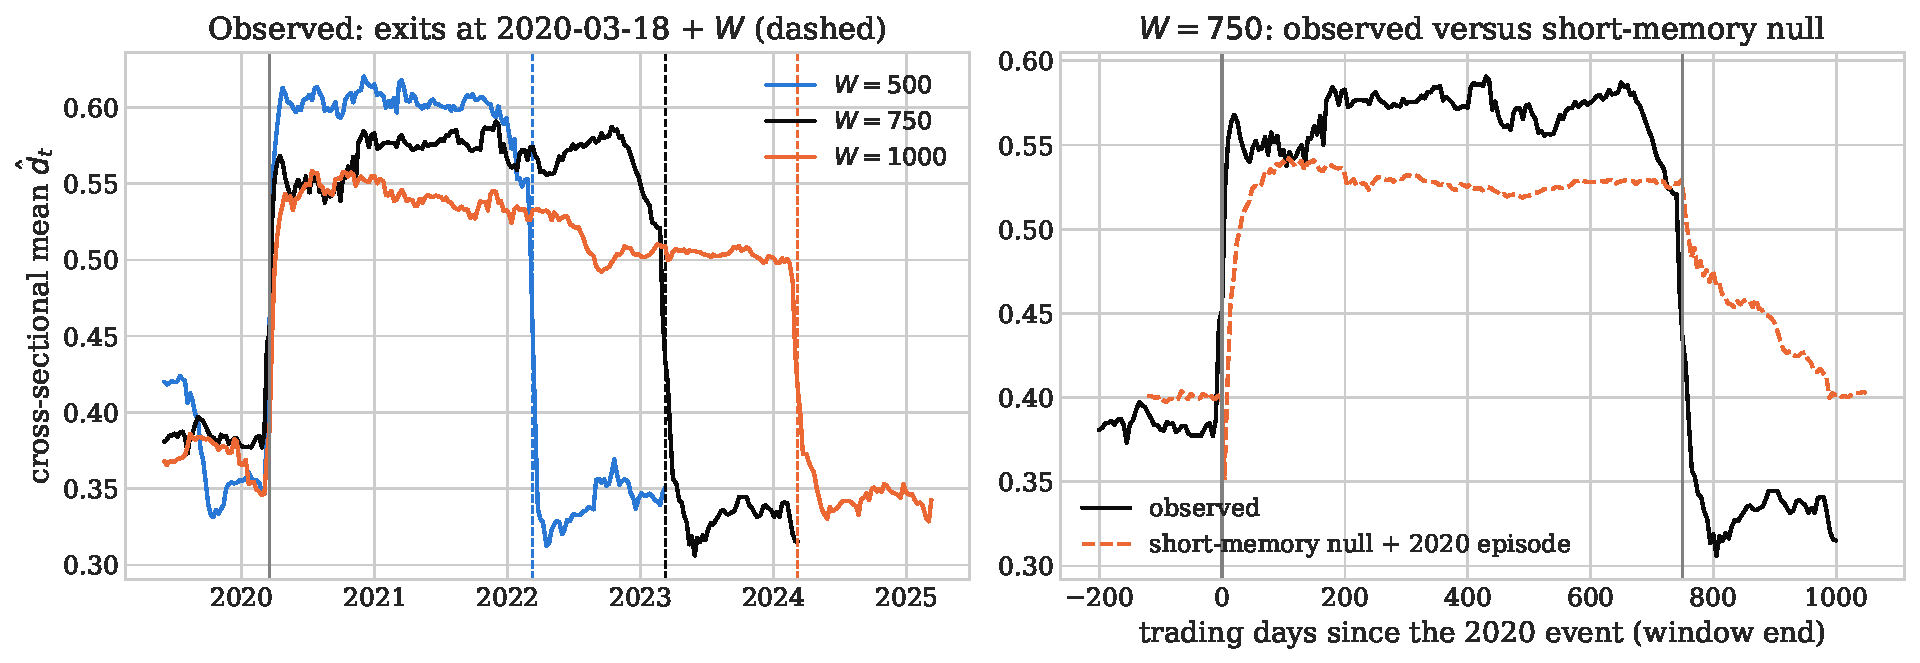
\includegraphics[width=\textwidth]{figures/fig10_window_inclusion.pdf}
\caption{The persistence state around the 2020 episode. Left: cross-sectional
mean of the rolling GPH estimate for windows of 500, 750 and 1000 trading
days; the solid gray line marks 18 March 2020 and the dashed lines the dates
on which that day leaves each window. Right: the 750-day series in event
time and the mean of 200 simulations of a short-memory ARMA(1,1) process,
fitted to 2012--2019 data, with the observed 2020 excess log variance
added.}
\label{fig:window}
\end{figure}

Panel C and the right panel of Figure~\ref{fig:window} ask whether a process
without long memory can generate this pattern. We fit an ARMA(1,1) model to
each stock's log variance over 2012--2019, a period without an episode of
the scale of 2008 or 2020, take the median parameters ($\phi=0.91$,
$\theta=-0.69$), add the observed cross-sectional median excess log variance
of the year after 18 March 2020, and apply the same rolling estimator to 200
simulated paths. The simulated state starts at 0.40, close to the observed
0.385, rises on entry, holds a plateau, and has its largest fall within nine
days of the exit date at every window length. It reproduces 53--69\% of the
observed rise. A shortfall is to be expected, since the null contains a
single stylized episode with the cross-sectional median profile, whereas each
stock's window in the data also contains its own later shocks of 2020--2022.

\subsection{Implications}

Two implications matter for what follows. First, a persistence state built
from rolling long-memory estimates is a lagged and smoothed record of how
much extreme volatility has occurred over the past few years. Implied
volatility already reflects that history, partly through the variance risk
premium, which rises after crises and decays slowly \citep{bates2000post,
andersen2015risk}. There is therefore little reason to expect the state to
add forecasting information, and Sections~\ref{sec:results} and
\ref{sec:robust} find that it does not.

Second, rolling memory estimates should not be read as evidence of changing
persistence or efficiency without checking how their turning points depend on
the window. The dates illustrate the risk. With a 750-day window the 2020
shock leaves the window on 10 March 2023, the day Silicon Valley Bank
failed; with a 500-day window it leaves on 11 March 2022, two weeks after
Russia invaded Ukraine. A study based on a single window could plausibly
attribute the fall in persistence to one of those events. Varying the window
and checking whether the turning points move with it is an inexpensive
safeguard. Our evidence concerns memory in volatility; whether rolling
estimates of memory in returns behave in the same way depends on the
estimator and is left for future work.
